%%%%%%%%%%%%%%%%%%%%%%%%%%%%%%%%%%%%%%%%%%%%%%%%%%%%%%%%%%%%%%%%%%%%%%%%
% RevTeX 4.1 LaTeX
% Kevin C. Young
% Scalable & Secure Systems Research (08961)
% Thu Mar  5 15:29:19 PST 2015
%%%%%%%%%%%%%%%%%%%%%%%%%%%%%%%%%%%%%%%%%%%%%%%%%%%%%%%%%%%%%%%%%%%%%%%%

\documentclass[aps,nofootinbib,pra,notitlepage,twocolumn]{revtex4-1}
\usepackage{amsfonts,amsmath,amssymb,amsthm}
 \usepackage{array,bm,color}
\usepackage{epsfig,graphicx,nomencl,revsymb4-1,upgreek,url}
\usepackage{hyperref}
\usepackage{algorithm}
\usepackage{algpseudocode}
\usepackage{graphicx}
\graphicspath{{./figures/}}
\hypersetup{colorlinks=true, pdfauthor=Kevin C. Young, pdftitle=Decorrelating Errors}
\newcommand{\tr}{{\rm Tr\thinspace}}
\newcommand{\bra}[1]{\ensuremath{\left\langle{#1}\right\vert}}
\newcommand{\ket}[1]{\ensuremath{\left\vert{#1}\right\rangle}}
\newcommand{\braket}[2]{\left\langle #1 | #2 \right\rangle}
\newcommand{\ketbra}[2]{\left| #1 \right\rangle\!\!\!\,\left\langle #2 \right|}
\newcommand{\abs}[1]{\left\vert #1 \right\vert}
\newcommand{\expect}[1]{\ensuremath{\left\langle{#1}\right\rangle}}
\newcommand{\timeorder}{\ensuremath{\underset{\leftarrow}{\mathcal{T}}}}
\newcommand{\ident}{{\mathbb1}}
\newcommand{\order}[1]{\mathcal{O}\left( #1 \right)}
\newcommand{\diag}[1]{\mathrm{diag}\{#1\}}
\newcommand{\trans}[1]{#1^\mathsf{T}}
\newcommand{\T}{\mathsf{T}}
\newcommand{\erf}[1]{Eq.~(\ref{#1})}
\newcommand{\needcite}{{\color{blue}\textsuperscript{[citation needed]}}}
\newcommand{\note}[1]{{\color{red}[#1]}}
\newcommand{\kcy}[1]{{\color{red}[#1]_{\rm{KCY}}}}
\newcommand{\amp}[1]{{\color{red}[#1]_{\rm{AMP}}}}

\newcommand{\actual}{\ensuremath{\tilde{\mathcal{G}}}}
\newcommand{\target}{\ensuremath{{\mathcal{G}}}}
\newcommand{\error}{\ensuremath{{\mathcal{E}}}}

%-------------Header begins here----------------------------------------
\begin{document}
\title{Advantages of mixed unitary operators for quantum information processing}

\author{Anthony M. Polloreno}
\email[Email: ]{anthony@rigetti.com}
\affiliation{Rigetti Computing, Berkeley, CA}

\author{Kevin C. Young}
\affiliation{Sandia National Laboratories, Livermore, CA}

\date{\today}

\begin{abstract}
...
\end{abstract}

\pacs{}

\maketitle


% ==============================================================================
% Section: Introduction
% ==============================================================================
\section{Introduction}
\label{sec:introduction}

The past decade has seen a dramatic increase in the performance and scale of quantum information processors (QIPs). Gate fidelities are now routinely in the 99\% to 99.99\% range \cite{Barends2014, Ballance2016}, and dozens of individually-addressable qubits are becoming available on integrated devices. While these advances represent important steps forward on the path towards a computationally useful QIP, the quantum advantage milestone \cite{1203.5813} has yet to be definitively reached. The limiting factor, of course, is errors in the quantum gate operations.

The impact of an error in a quantum gate depends strongly on both the magnitude and the nature of the errors. Systematic, or \emph{coherent}, errors can arise from poorly calibrated controls or imperfect gate compilations that induce repeatable, undesired unitary errors on the state of a QIP. Errors of this type are correlated in time and add up coherently. They are are  computationally expensive to model and it is difficult to place analytic bounds on circuit performance. Contrast this against random, or \emph{stochastic}, errors, which result from high-frequency noise in the controls or the environment. Systems with stochastic errors can be  modeled by defining a rate of various discrete errors in the system, such as a bit flip or phase flip. These errors are significantly easier to simulate on a classical computer, and their impact on quantum circuits is much easier to estimate.

Despite the relative ease of modeling stochastic errors, coherent errors are often much more likely to appear in QIPs. Drifting control parameters or environmental variables can easily have long correlation times that result in errors which is strongly coherent over the length of a quantum circuit. While these errors can often be reconstructed using various tomographic techniques, their impact is difficult to predict. The diamond distance can be used to estimate the failure probability of a quantum circuit, but the diamond distance can grow quadratically with repeated application of gate with coherent errors. For long circuits, this can add up extremely quickly. Recent work by Hastings and Campbell\cite{Campbell2017, 1612.01011, 1811.08017}, however, has shown that coherent noise can be strongly suppressed by probabilistic sampling over various implementations of the target quantum gates. This averaging results in quantum processes with diamond distances that grow only linearly  quadratic in the over/under rotation angle of the component gates. \note{Clear this up.}

In this article we discuss various applications of mixed unitary controls, and show that the advantages of this approach can be made robust to drift in the target gates. We present an optimal control approach to the mixed unitary control design problem. We apply our methods in simulation where we construct single- and two-qubit mixed unitary controls which are robust to drift and uncertainty in the control parameters. We further present an experimental implementation of single-qubit mixed unitary controls on a superconducting qubit testbed at Rigetti Quantum Computing. Using randomized benchmarking, we are able to show a marked improvement in error rates, as well as a reduced variance in circuit outcome probabilities, indicating a reduction in the coherence of the error.

% For instance, the repeated measurements that occur in quantum error correction are suspected to reduce the potential impact of coherent buildup of error. Modern devices, however, do not have sufficient numbers of qubits and their errors are above the threshold at which QEC becomes a viable option.


% ==============================================================================
% Section: Mathematical preliminaries
% ==============================================================================
\section{Mathematical preliminaries}
\label{sec:representing_quantum_gates}
Quantum gate operations are implemented by applying a sequence of classical control fields to some set of qubits. Fluctuations in the environment or imperfections in the controls can cause the state of the qubits to change in a way that is different from what was intended.  But if the gates are fairly stable with time and context, then we can describe their action on the qubit state using \emph{process matrices}, linear, Markovian maps on the state of some qubits.  When working with process matrices, it is convenient to write the system density operator using a vectorized representation, and in this article, we'll make use of the generalized Bloch vector,
\begin{equation}
  \vec \rho = \tr(\rho \vec \Sigma),
\end{equation}
where $\vec \Sigma$ is a vector of all $4^n$ $n$-qubit Pauli operators. The action of a gate is then given by the usual matrix multiplication:
\begin{equation}
  \rho \rightarrow \target\rho = \error \actual \rho.
\end{equation}
Here $\target_i$ is the target operation, $\actual$ is the actual gate as implemented, and $\error$ is the effective error channel. 
 
\begin{equation}
	\left(\begin{array}{c|cccc}
		1 &  & \vec0 & \\ 
		\hline & &  &  \\
		\vec{m} &  & R &  \\
		 &  &  & 
	\end{array} 	
	\right)
\end{equation}

The top row of all trace-preserving (TP) maps is fixed to $\{1,0,0,0,\cdots\}$.  The rest of the first column, $\vec{m}$, describes any deviations from unitality, such as could arise from amplitude damping. If the error channel is unitary, then the error is coherent, and the submatrix $R$ is perfectly antisymmetric, corresponding to a rotation of the generalized Bloch vector. If  $R$ is diagonal, then the error channel is Pauli stochastic, with each entry corresponding to the probability that the associated Pauli error occurs in each application of the gate. \note{Be more clear about what "associated" means here}.  If R is symmetric but not diagonal, then the channel is still stochastic, but the random errors consist of correlated Pauli operators (such as $X+Y$). For a single qubit, this describes everything, but the situation can be slightly more complicated for more qubits. 

The channel that results is:
\begin{align}
	\mathcal{M} 
		=& \sum_i p_i U^*_i \otimes U_i \\
		=& \sum_i p_i \exp(i \frac{\theta}{2}\hat n \cdot \vec\sigma^*) \otimes \exp(-i \frac{\theta}{2} \hat n \cdot \vec\sigma) \\
		=& \sum_i p_i (\cos\theta + i \sin\theta H^*)\otimes(\cos\theta -i \sin\theta H) \\
		=& \sum_i p_i (\cos\theta^2 I\otimes I + \sin\theta^2 H^*\otimes H \\ & + i\sin\theta\cos\theta H^*\otimes I
								- i\sin\theta\cos\theta I\otimes H )
\end{align}
In this case, $\sin\theta^2$ is always positive, so we cannot hope to eliminate the second term, but $\sin\theta\cos\theta$ may be positive or negative, and so there is hope that we could possibly combine various implementations to eliminate this term. The result would be a purely stochastic channel. 


The \emph{size} of an error in quantum gates may  be quantified in a number of ways. Two of the most common metrics are the average gate fidelity, $\mathcal{F}$, and the diamond norm, $\vert\vert\cdot\vert\vert_\diamond$. These may be represented in terms of the error maps as
\begin{equation}
	\vert\vert \error \vert\vert_\diamond = \sup_\rho \vert \vert (I\otimes I)(\rho) - (\error \otimes I)(\rho) \vert\vert_1
\end{equation}
\begin{equation}
	\mathcal{F}(\error) = \frac{Tr(\error^*\otimes\error) + d}{d^2 + d}
\end{equation}
The diamond norm is generally linear in the over-rotation angle of a quantum operation, while the AGI is generally quadratic in the over-rotation angle of a quantum operation. 

A mixed unitary channel consists of a set of unitary channels, $\actual_i$, and associated weights, $\sum_i p_i = 1$.  The process matrices for a mixed unitary channel are then the weighted sum of the component channels, $\actual_{\rm M} = \sum_i p_i \actual_i$, and the associated error channel is simply the weighted sum of the associated error channels, $\error_{\rm M} = \sum_i p_i \error_i$. 

Campbell considered the very important problem of minimizing the diamond norm of the resulting error channel. Given a collection of component channels with error at most $\epsilon$, Campbell and Hastings gave a sufficient condition for the diamond norm to be minimized to first order in $\epsilon$. In their their mixing lemmas\cite{Campbell2017, 1612.01011}, they show that the Hamiltonians should form a convex set containing the origin. The diamond norm is a particularly appealing target, because the diamond norm provides useful error metrics on quantum circuits. However, it is not the only optimization target that can be chosen. If the ultimate goal is to produce a channel whose effect can be easily simulated, then it may be useful instead to construct a channel whose errors are Pauli stochastic. Such a channel could be produced by instead minimizing the off-diagonal elements of the process matrix.

%\eq

% ==============================================================================
% Section: Example Mixed Unitary Processes
% ==============================================================================
\section{Example Mixed Unitary Processes}
\label{sec:mixed_unitary_processes}
There are often many possibly ways of implementing any given target quantum gate. Hastings and Campbell, for instance, consider gates compiled using the Solovey-Kitaev algorithm, for which  many approximate gate compilations are possible. By selecting from these various implementations at random, they show that the resulting quantum channel can be made to have significantly reduced coherent error. As a simple example of how this occurs, consider a scenario in which we have a single-qubit and four possible implementations of a $\pi$-pulse about the $\sigma_x$ axis. The error channels for these four implementations are themselves unitary rotations about the $\sigma_x$ axis with rotation angles of $\{-2\epsilon, -\epsilon, \epsilon, 2\epsilon\}$. Such a situation could appear, for instance, if there were amplitude errors on the fields used to affect the gates, and if the control could be implemented by a rotation about the positive or negative $\sigma_x$ axis.

\begin{center}

\begin{tabular}{cccc}
	Gate & $H_{\rm{eff}}$ & AGI & $\vert\vert\cdot\vert\vert_\diamond$ \\
\hline
	$U_{+2\epsilon}$ & $2\epsilon \sigma_x$ & $4\epsilon^2$ & $2\epsilon$\\
	$U_{+\epsilon}$ & $\epsilon \sigma_x$ & $\epsilon^2$ & $\epsilon$ \\
	$U_{-\epsilon}$ & $-\epsilon \sigma_x$ & $\epsilon^2$ & $\epsilon$ \\
	$U_{-2\epsilon}$ & $-2\epsilon \sigma_x$ & $4\epsilon^2$ & $2\epsilon$ 
\end{tabular}

\end{center}


\begin{figure}
  \centering
  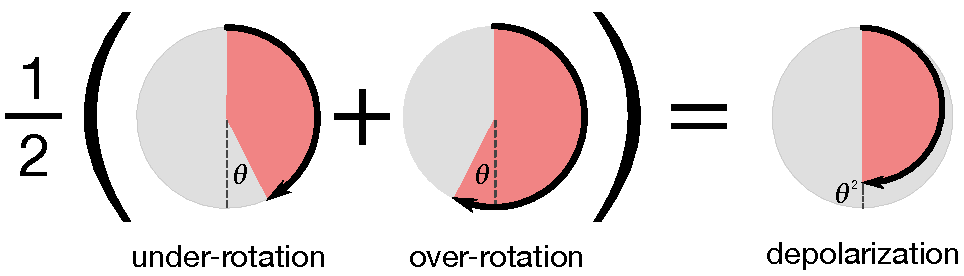
\includegraphics[width=\columnwidth]{simple_example.pdf}
  \caption{An example of a mixed unitary process. Using optimal control, two implementations of a $Z_\pi$ gate are designed to have equal and opposite sensitivity to errors (if one implementation over-rotates by angle $\theta$, then the other \emph{under}-rotates by $\theta$). Each time the gate is used, one of these implementations is chosen at random. The resulting quantum channel is equivalent to a perfect implementation of the gate followed by dephasing of $\order{\theta^2}$.}
  \label{fig:simple_example}
\end{figure}

In this case, the MUP that minimizes the diamond norm is given by:
\begin{equation}
\frac{1}{2}U_{+\epsilon}^*\otimes U_{+\epsilon} + \frac{1}{2}U_{-\epsilon}^*\otimes U_{-\epsilon}
\end{equation}
Additionally, it is clear that because the AGI is linear, the AGI of any convex weighting of these two channels will be $\epsilon^2$.
\note{This example is really useful and should be expanded. We should discuss the various optimization problems, a mixed unitary strategy, the fidelity of the resulting channel.}



% ==============================================================================
% Section: Robustly Mixed Unitary Processes
% ==============================================================================
\section{Robustly Mixed Unitary Processes}
\label{sec:robustly_mixed}
\note{Decide on naming convention, Anthony has used $\ell$ MUP in the rest of the text} 

\note{Anthony references this section when discussing minimizing the offdiagonal elements of the error's process matrix.}

While mixed unitary processes offer significant improvements to gate performance, they fail to take into account the reality that most control electronics experience drift over time scales relevant to QIP performance. Because of this drift, the quality of the MUP will degrade. Thus, we would like to design mized unitary processes that are \textit{robust} to this drift. A mixed unitary process is said to be robust to order $\ell$ if for all $1 \leq j \leq \ell$:
\begin{equation}\label{eq:MUP}
\begin{gathered}
\sum_k\omega_k(\sum_{n=0}^j D^n_k)^j = 0\\
D^n_k = \frac{1}{n!}\frac{\partial^{n}}{\partial\delta_{i_1}...\partial\delta{i_n}}H_k(t,\vec{\delta})|_{\delta=\vec{0}}
\end{gathered}
\end{equation}
These conditions imply that an $\ell^{th}$ order MUP ($\ell$MUP) is insensitive to the $\ell^{th}$ order in drift in $\vec{\delta}$. To see this, write the error on each gate in the MUP as 
\begin{equation}\label{eq:taylor}
\begin{gathered}
U_j(\vec{\delta}) = exp(-i(\tilde{H}_j(\vec{0}) + \frac{\partial}{\partial\delta_i}\tilde{H}_j(d\delta_i)\\ +  \frac{1}{2}\frac{\partial^2}{\partial\delta_i\partial\delta_k} \tilde{H}_j(d\delta_i d\delta_k) + ...)U_T
\end{gathered}
\end{equation}
where $\tilde{H}(\delta)$ generates the error $U_j(\vec{\delta})U_T^{\dagger}$ over variations in $\vec{\delta}$. Then, by Taylor expanding $U_j(\vec{\delta})U_T^{\dagger}$ one finds that the the first $\ell$ derivatives of an $\ell RBC$ will be zero.

Following from Lemma 2 in \cite{Campbell2017}, if $0\in $ Conv$[\{\tilde{H}_i(t, \vec{\delta})\}]$, where Conv is the convex hull of its arguments, then we know that $\vec{\omega}$ exists that quadratically decreases the diamond norm. Then, following from the mixing lemma proven by both Campbell and Hastings\cite{1612.01011}, we can bound the the diamond distance from a balanced control to $U_T$ by $\epsilon^2$. We can relax Equation \ref{eq:MUP}, to be
\begin{equation}\label{eq:RBC-relaxed}
\begin{gathered}
\sum_k\omega_kD^n_k = 0\\
\end{gathered}
\end{equation}
In this context, since we are assuming that the derivatives are all of norm $\epsilon$, the above condition guarantees that the error unitary be no worse than $\sum^n\epsilon^2\delta^n$ near the origin -- all orders can be quadratically supressed. Figure \ref{fig:vectorspace} gives geometric intuition for robustly mixed unitary processes.

\begin{figure}
  \centering
  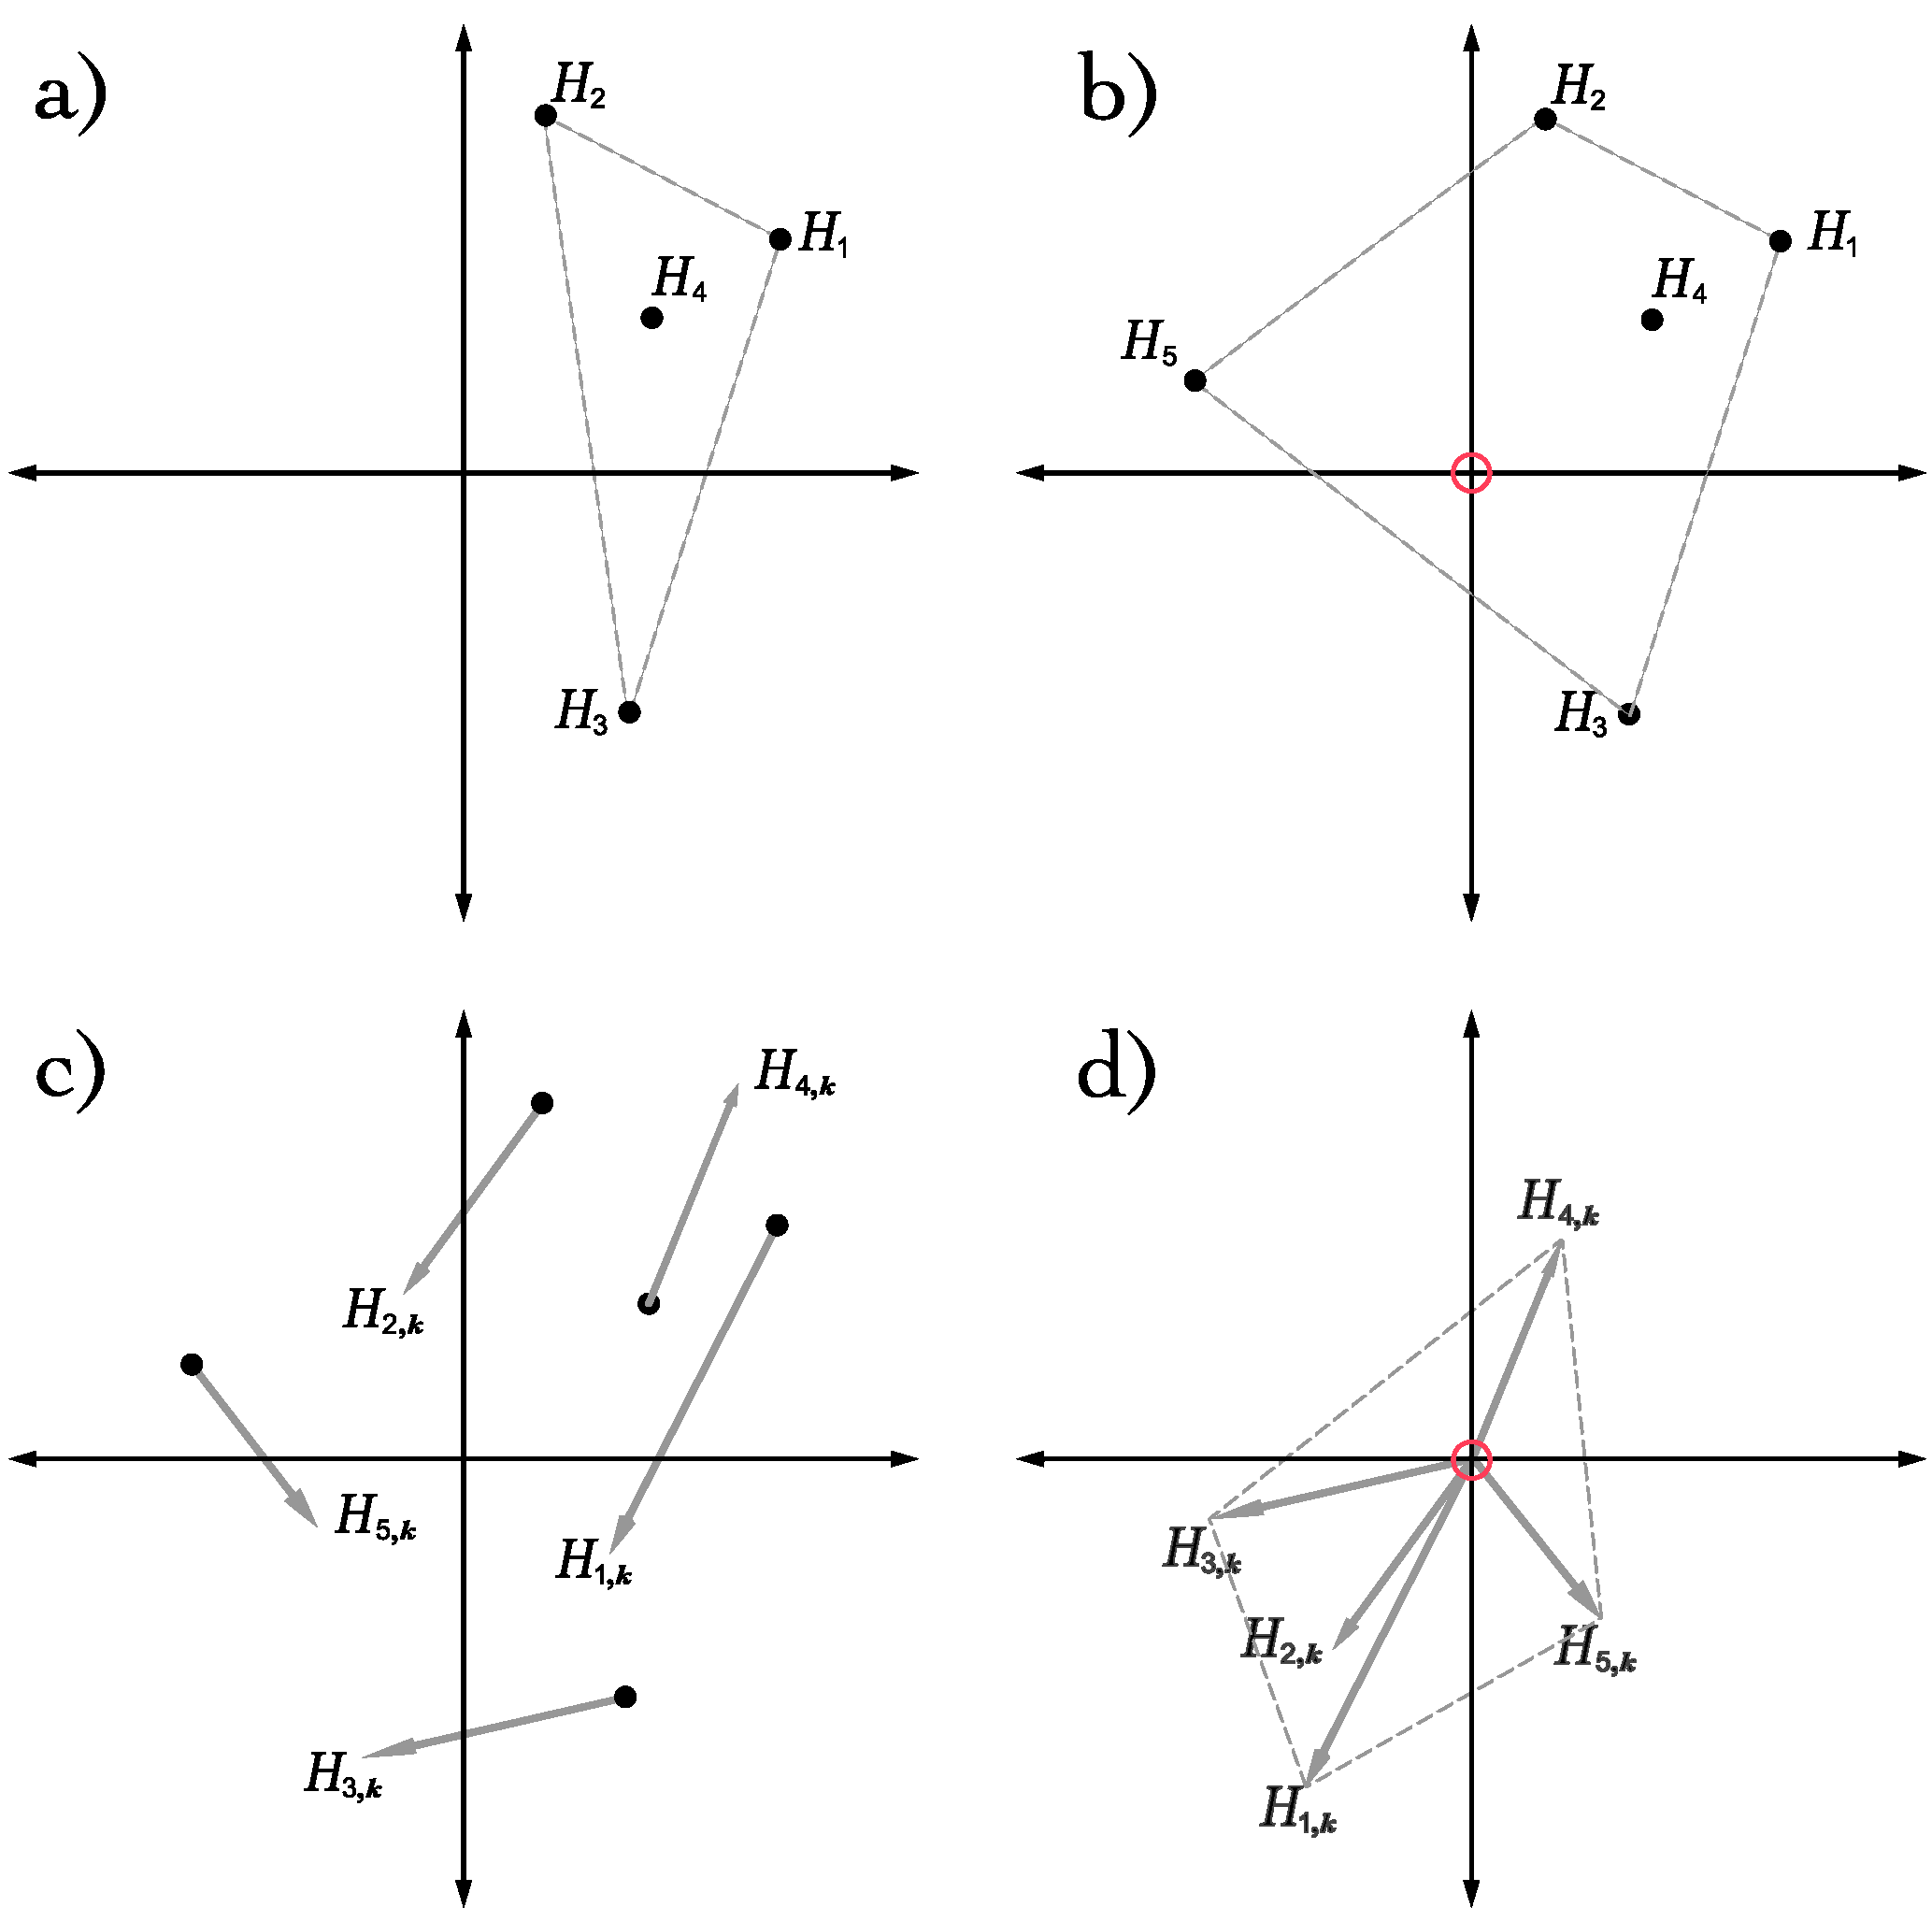
\includegraphics[width=\columnwidth]{vectorspace.pdf}
  \caption{A target unitary gate can be implemented a number of ways, each with a different effective Hamiltonian error. These error Hamiltonians lie in a vector space. a) Four effective Hamiltonians. The origin is not contained in their convex hull, so there are no balanced control solutions. b) The origin is contained in the covex hull after adding an additional control solution. Because there are more than $n+1$ implementations, there exist an infinite number of balanced control solutions. c) The error Hamiltonians shown with their derivative with respect to a control parameter. As this parameter drifts, a $0^{\rm th}$-order balanced control solution may drift, leading to a first-order error. d) The derivatives also lie in a vector space. If the origin lies in their convex hull, then it may be possible to construct a $1^{\rm{st}}$-order robust balanced control solution.}
  \label{fig:vectorspace}
\end{figure}


% ==============================================================================
% Section: Generationg of Robustly Mixed Unitary Processes
% ==============================================================================
\section{Generation of Robustly Mixed Unitary Processes}
\label{sec:generation}

\subsection{Random Gate Synthesis}
\label{sec:random_gate_synthesis}
 In this article, we use optimal control to generate the one qubit families of controls for MUPs. One could use any of the many available quantum optimal control techniques \cite{Khaneja2005, Caneva2011, Machnes2018}, and for our numerics we chose to use the GRAPE algorithm. First described in \cite{Khaneja2005}, the GRAPE (GRadient Ascent Pulse Engineering) algorithm is a technique for finding piecewise constant control sequences that approximate a desired unitary, $U_T$, given a Hamiltonian with controlled and uncontrolled terms. Defining the uncontrolled Hamiltonian as $H_0$, the control Hamiltonians as $H_{i\neq 0}$, and the \textit{control matrix} $c_{ij}$ as containing the control amplitude associated with the $i^{th}$ time step and the $j^{th}$ Hamiltonian, we can write an the unitary for any timestep of evolution as:
\begin{equation}\label{eq:3}
  U_i = \exp\{-i\Delta t(H_0 + \sum_{j=1}^{n}c_{ij}H_{j}\}
\end{equation}
To measure the simularity of our approxiate unitary $U=\prod_iU_{i=1}^n$ to our target unitary $U_T$, we can define a cost function $J(U) = Tr\{U_T^{\dagger}U\}$.

To optimize this cost function we can perform the following standard update loop for some threshold value $\varepsilon > 0$ and step size $\delta > 0$:
\begin{algorithm}[H]
\floatname{algorithm}
  \caption{\textsc{\textbf{Gradient Ascent}}}
  \begin{algorithmic}
    \While{$J(U) < (1-\varepsilon$)}
    \State $c_{ij} \rightarrow c_{ij} + \delta\frac{\partial J(U)}{\partial c_{ij}}$
    \For{$1 \leq i \leq n$}
    \State $U_i \rightarrow \exp\{-i\Delta t(H_0 + \sum_{i=0}^{n}c_{ij}H_j)\}$
    \EndFor
    \State $U \rightarrow \prod_{i=1}^nU_i$
    \EndWhile
  \end{algorithmic}
\end{algorithm}

In general these gradients can be computed by propagating partial derivatives of the cost function with respect to control parameters through each timestep of the  via the chain rule. However, in \cite{Khaneja2005} Khaneja et al. derive an update formula that is correct to first order, and efficient to compute. In particular one can show that:
\begin{equation}\label{eq:update}
  \begin{split}
\frac{\partial J(U)}{\partial u_{ij}} = -2Re\{\braket{{U_{j+1}^{\dagger}...U_N^{\dagger} U_T}}{i\Delta tH_jU_j...U_1}\\
\braket{U_j...U_1}{U_{j+1}^{\dagger}...U_N^{\dagger} U_T}\} +  \mathcal{O}(\Delta t^2)
  \end{split}
\end{equation}

Because we our trying to generate high-order RBCs, we want to generate controls that perform well even in the presence of drift. To do this, we modified the gradient in GRAPE to instead be:
\begin{align}\label{eq:quadrature}
\frac{\partial \tilde J(U)}{\partial u_{ij}} =
\int p(\vec{\delta})\frac{\partial J(U(\vec{\delta}))}{\partial u_{ij}} d\vec{\delta}
\end{align}
with $p(\vec{\delta})$ Gaussian distributed, as has been done in previous works \cite{Goerz2014} to ensure that the optimal control results are robust over a wide range of errors. To make this averaging tractable, we approximate this integral using Gaussian quadrature, approximating the cost function as a low order polynomial\cite{abramowiz1972handbook} (in particular degree 5). Note that despite updating the gradient, we did not change the cost function. The termination condition for the gradient ascent loop is still just that the controls perform well in the absence of drift. This is not a fundamental requirement of the routine, but rather was done to make finding solutions with $J(U) < 1 - \epsilon$  less computationally taxing.

\subsection{Optimal Weighting}
To generate robustly mixed unitary processes, we can solve the following convex optimization problem:

\begin{equation}\label{eq:minimization}
  \begin{split}
    &\underset{\omega_j\geq0, |\omega|_1=1}{\textbf{minimize}: } ||D_{\ell}^T\omega||\\
    &\textbf{subject to: } \forall i<\ell, \sum \omega_jD_j^i=0\\
  \end{split}
\end{equation}

If the control family is too small a solution won't exist, in particular as in \cite{Campbell2017} we need  $0\in $ Conv$[D_j^i]$.  This can be accomplished by modifying the oracle in Campbell's algorithm to produce robust controls, in particular by updating the GRAPE cost function to include derivative information, one could produce controls with derivatives of order $\epsilon$. In our case, by using the Gaussian weighted cost function, we ensure that the controls generated should have vanishing first derivative.

This minimization problem, while sufficient for quadratically decreasing the diamond norm relative to the \textit{worst} controls in the family, does not preferentially select the controls with the least error. That is to say, as in Section \ref{sec:mixed_unitary_processes}, both \{$U_{+2\epsilon}$, $U_{-2\epsilon}$\} and \{$U_{\epsilon}$, $U_{-\epsilon}$\} minimize this cost function for a 0MUP. To encourage the inclusion of controls with smaller error, we may impose an $\ell_2$ penalty to our cost function by rewriting it as:

\begin{equation}\label{eq:minimization_l2}
  \begin{split}
    &\underset{\omega_j\geq0, |\omega|_1=1}{\textbf{minimize}: } ||D_{\ell}^T\omega||_2 + \eta\sum||D_0^T\omega||_2\\
  \end{split}
\end{equation}
with $\eta \geq 0$. 

To make sure the routine remains practical, we would also like to regularize our objective function to enforce sparsity. In this case, lasso regularization \cite{tibshirani1996regression} is insufficient as we already constrain the one norm of the vector we optimize over to be one. However, the problem of enforcing sparsity in such situations has been considered in \cite{NIPS2012_4504} and can be expressed via another convex program that extends Equation \ref{eq:minimization}:
\begin{equation}
\begin{split}
\underset{n\in[N]}{\textbf{minimize}}\{
    &\underset{\omega_j\geq0, |\omega|_1=1, t\geq0}{\textbf{minimize}: } ||D_{\ell}^T\omega|| + t\\
    &\textbf{subject to: } \omega_n > \frac{\lambda}{t}\\
    &\phantom{\textbf{subject to: }} \forall i<\ell, \sum \omega_jD_j^i=0\}
\end{split}
\end{equation} where $\lambda$ is a hyperparameter to be optimized over.


% ==============================================================================
% Section: Numerical Results
% ==============================================================================
\section{Numerical Results}
\label{sec:numerical_results}
In the following numerical results, we explore using the methods in Section \ref{sec:mixed_unitary_processes} to build MUPs. We consider the following model for a single tunable qubit: 
\begin{equation}\label{eq:1Qham}
  H(\delta, \epsilon, t) = \epsilon\sigma_z + (1 + \delta)(c_x(t)\sigma_x + c_y(t)\sigma_y)
\end{equation}
We use the GRAPE algorithm as discussed in Section  \ref{sec:random_gate_synthesis} with N=25 steps and total evolution time of $\pi$ to generate 100 candidate controls, with a standard deviation of $\sigma=.001$ for the distribution in Equation \ref{eq:quadrature}. We assume that the errors on $\sigma_x$ and $\sigma_y$ are perfecly correlated, as is the case in systems that implement RZ rotations with phase shifts of the control signal. Solving the optimization problem defined in Section \ref{sec:robustly_mixed} yields similar MUPs for $RX(\frac{\pi}{2})$ and $RY(\frac{\pi}{2})$, with the results for $RY(\frac{\pi}{2})$ shown in Figure \ref{fig:YMUP}. These results demonstrate several properties that make MUPs both useful and tractable.

\begin{figure*}
  \centering
  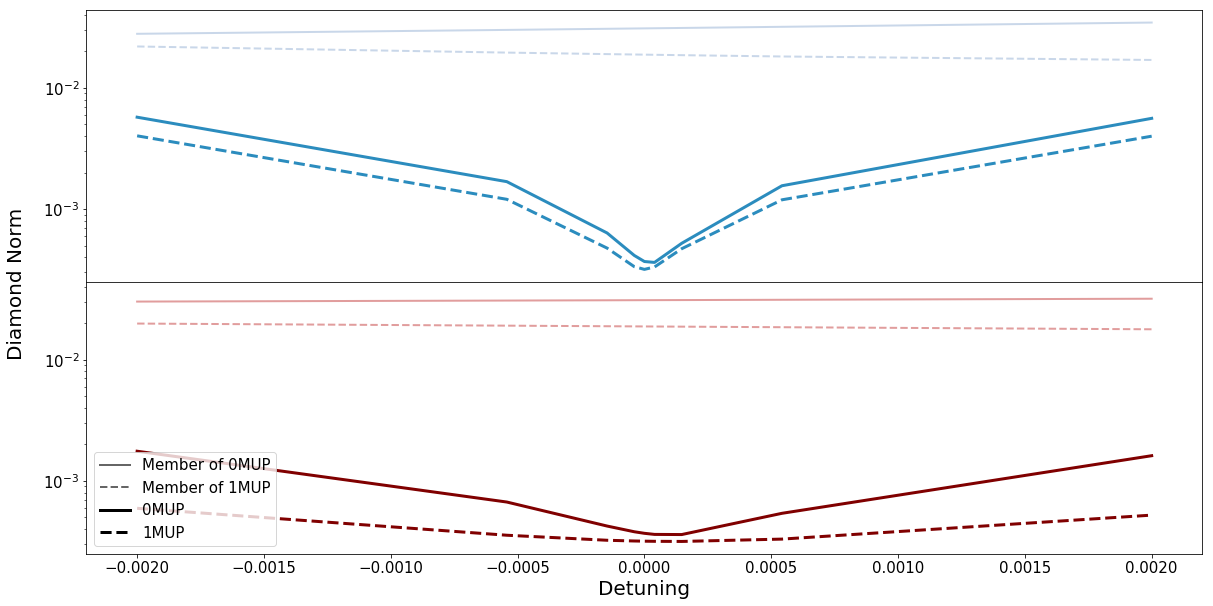
\includegraphics[width=\textwidth]{SQRTY.png}
  \caption{Numerical results comparing a 0MUP to a 1MUP for a single tunable qubit, for $RY(\frac{\pi}{2})$. The results are quantitatively similar to those for $RX(\frac{\pi}{2})$, but in this case the 0MUP is worse at the origin. This can be improved by penalizing for the norms, or by simply trying to find a 1MUP, which both symmeterizes the performance at the origin and makes them better.}
  \label{fig:YMUP}
\end{figure*}

%\begin{figure*}
%  \centering
%  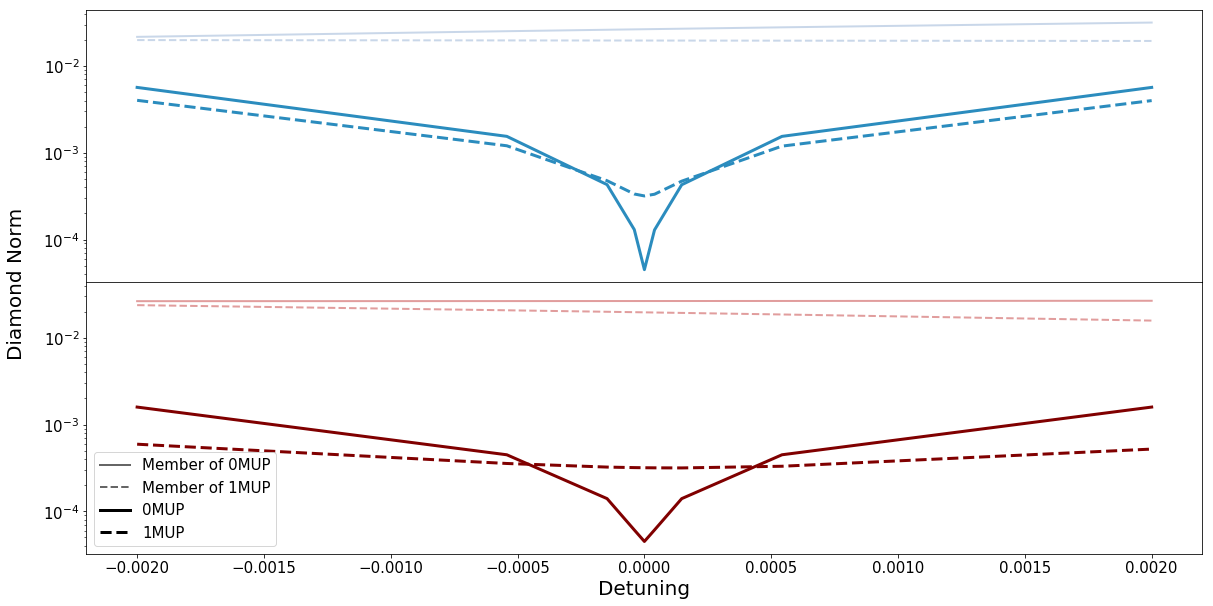
\includegraphics[width=\textwidth]{SQRTX.png}
%  \caption{Numerical results comparing a 0MUP to a 1MUP for a single tunable qubit, for $RX(\frac{np.pi}{2})$. Shown with lower alpha values are example members of the control families, with diamond norms of around $10^{-2}$. The 0MUP can be seen to outperform the members of the control family by two orders of magnitude at the origin, and the 1MUP by an order of magnitude. However, the 1MUP can be seen to be flatter. In paritcular, for small detunings, the 1MUP performs better than the 0MUP.}
%  \label{fig:XMUP}
%\end{figure*}


First, naively generating a 0MUP results in nontrivial support on all the members of the control family. However, by rewriting the minimization to impose the sparsity constraint discussed in Section \ref{sec:robustly_mixed}, we can generate a 0MUP that uses just five of the controls. This shows that through adding constraints to our optimization routine, we can make the MUP practically useful. In both cases we impose the same $\ell_2$ penalty as described in Section \ref{sec:robustly_mixed}, so that the algorithm preferentially selects controls with smaller errors. Imposing this constraint allows us to trade off flatness at the origin for performance.

In our two-qubit example we consider the following model for two tunable qubits coupled by a resonant exchange interaction, similar to that in \cite{McKay2016}:
\begin{equation} \label{eq:2Qham}
\begin{split}
H(\vec{\delta}, \vec{\epsilon}, t) = &\sum_{j=1}^2(\epsilon_j\sigma_z^j + (1 + \delta_j)(c_x^jx(t)\sigma_x^j + c_y^j(t)\sigma_y^j)) \\
&+ \frac{1}{10}(XX + YY)
\end{split}
\end{equation}

In this example it was infeasible to use GRAPE to return non-trivial solutions. Instead we manually selected piecewise constant echoing sequences with 500 steps and total evolution time of $\frac{5\pi}{2}$. In particular, we considered $RX(\pi)$, $RX(-\pi)$, $RY(\pi)$ and $RY(-\pi)$ bang-bang sequences \cite{bangbang}, consisting of all combinations of simultaneous $\pi$ pulses activated at multiples of $8$ steps from the beginning of the controls, and the same multiple of $8$ steps prior to the end of the controls. An example of such a control is given in Figure \ref{fig:bangbang}. To give the control family a variety of RF errors, we added on uniformly distributed errors to each $\pi$ pulse, between $-.25$\% and $.25$\%.


\begin{figure}
  \centering
  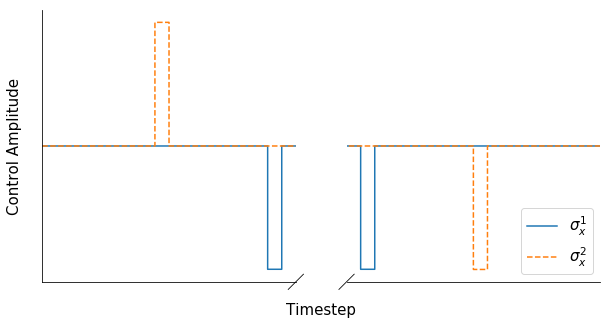
\includegraphics[width=\columnwidth]{bangbang.png}
  \caption{Example bang-bang sequence, using both qubits' $\sigma_x$ controls. Not shown are the $\sigma_y$ controls, and the uncontrolled resonant exchange interaction.}
  \label{fig:bangbang}
\end{figure}


In this example, we find more modest improvements to performance, as shown in Figure \ref{fig:2MUP}. There are now four free parameters to optimize over, and the uncontrolled entangling interaction means that there is little variation in the controls. Nonetheless, using a MUP improves performance by half of an order of magnitude at the origin, and up to an order of magnitude away from the origin, with the 1MUP performing just as well as the 0MUP, but also being more robust to drift. 


\begin{figure*}
  \centering
  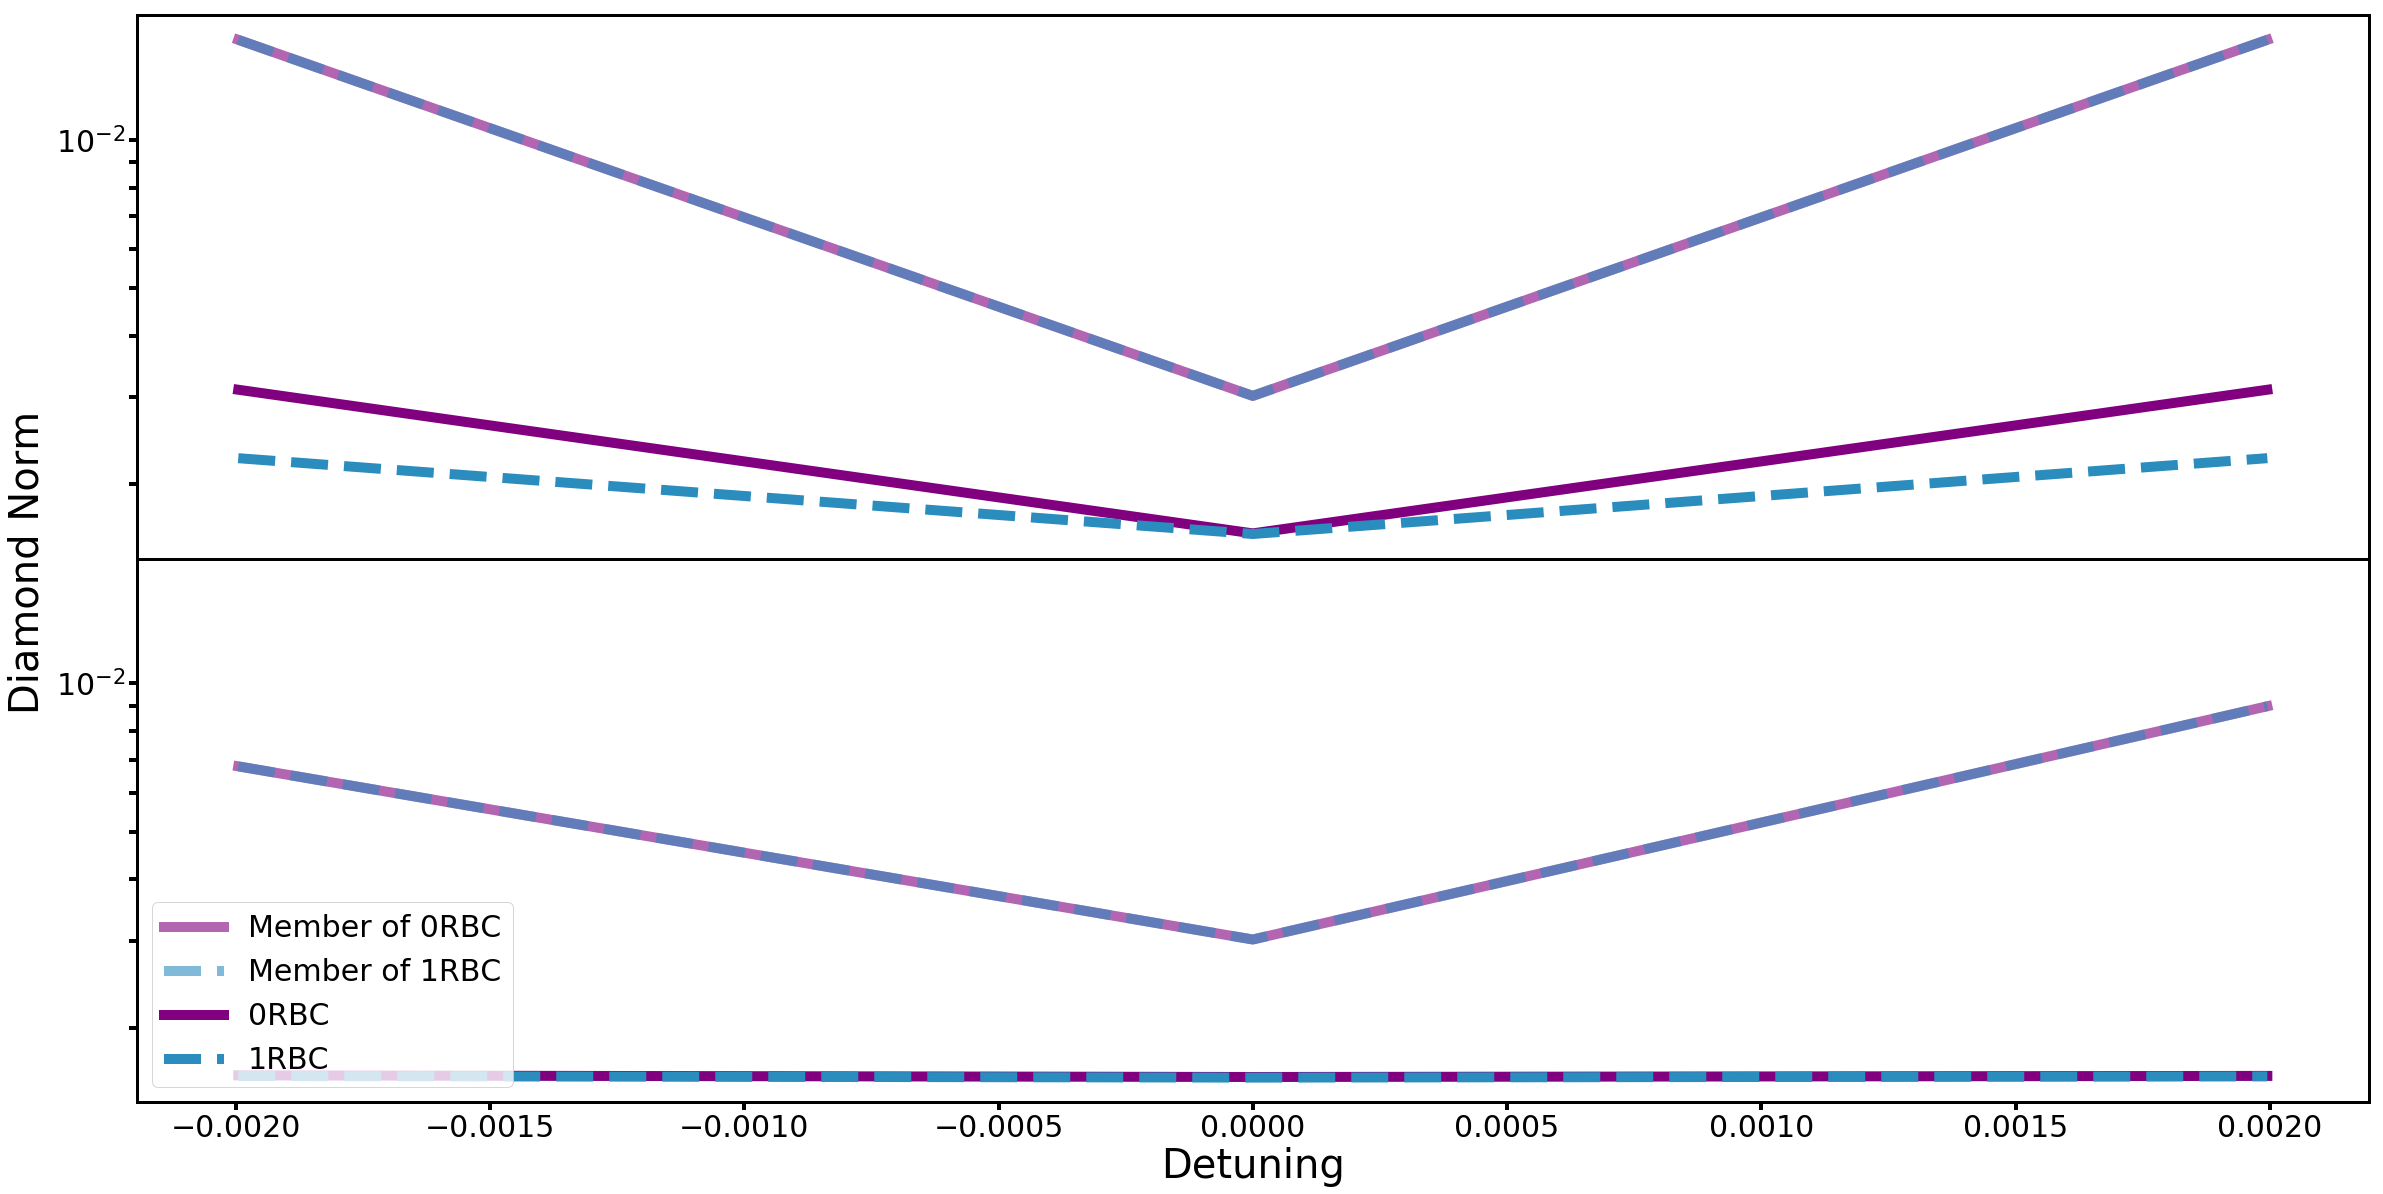
\includegraphics[width=\textwidth]{2QRBC.png}
  \caption{Numerical results comparing a 0MUP to a 1MUP for a pair of tunable qubits, with a resonant exchange interaction. Shown with lower alpha values are example members of the control families. The 0MUP and 1MUP can be seen to outperform the members of the control family by half an order of magnitude at the origin. Away from the origin, the 1MUP can be seen to be flatter. Far away from the origin, the 1MUP outperforms members of the control famlies by almost an order of magnitude in diamond norm.}
  \label{fig:2MUP}
\end{figure*}

% ==============================================================================
% Section: Experimental Results
% ==============================================================================

\section{Experimental Results}
\label{sec:experimental_results}
Here we present experimental results from implementing our routine on a fixed-frequency superconducting transmon qubit. In particular, we used qubit 8 on the Rigetti 19Q-Acorn chip, whose characterization can be found in \cite{1712.05771}. To implement a MUP on this qubit, four incorrectly calibrated Gaussian pulses were produced by scaling the pulseshape amplitude for a calibrated 10 sample 50ns $RX(\frac{\pi}{2})$ pulse by $106.4\%$,  $103.9\%$, $93.7\%$ and $91.2\%$.


\begin{figure}[H]
  \centering
  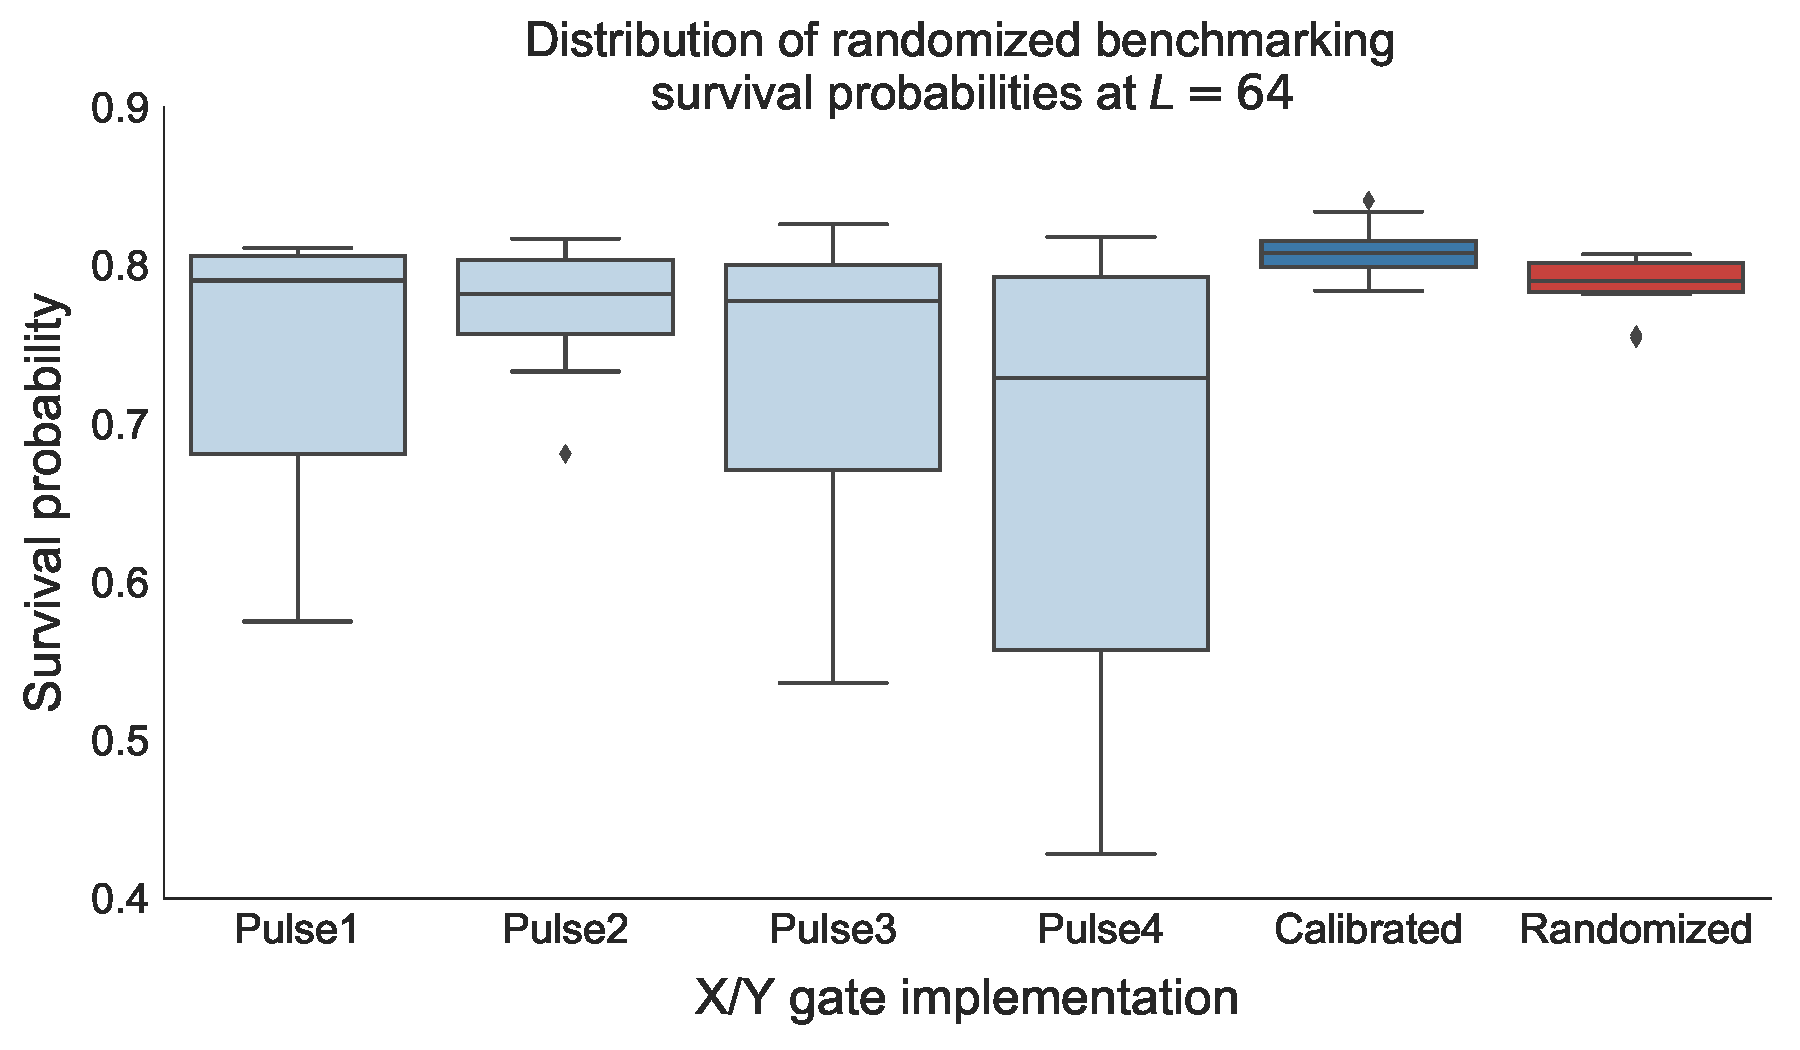
\includegraphics[width=\columnwidth]{rb_data.pdf}
  \caption{Randomized benchmarking experiments ran using different pulse definitions. The four plots on the left are from the incorrectly calibrated pulse, while the top right is the calibrated pulse, and the bottom right is the BCS.}
  \label{fig:rb}
\end{figure}


As discussed in Section \ref{sec:robustly_mixed}, we chose here to minimize the off diagonal elements of the process matrix. To benchmark the quality of the MUP, we then performed six randomized benchmarking experiments\cite{Magesan2011}: one for each over-- and under--calibrated pulse, one for the calibrated pulse, and one for the mixed process. We used $1000$ shots per experiment, $10$ sequences per sequence length, for sequence lengths of $2, 4, 8, 16, 32$ and $64$. In each case, our Clifford operations were decomposed into RX($\frac{\pi}{2})$) and RY($\frac{\pi}{2})$) pulses. In our implementation, these gates are implemented using the same pulse envelope definitions and control electronics, phase shifted by $\frac{\pi}{2}$ radians, and are therefore subject to identical miscalibration errors. The results are shown in Figure \ref{fig:rb} for sequence lengths $L=64$. Fitting to the randomized benchmarking decay curves, we find one-qubit gate fidelities of $99.3\%$ for the calibrated pulse, $98.9\%$ for Pulse1, $99.1\%$ for Pulse2, $98.9\%$ for Pulse3, $98.5\%$ for Pulse4, and $99.2\%$ for the MUP, demonstrating that it performs almost as well as the calibrated pulse, and better than the constituent pulses. 

Additionally, by minimizing the off-diagonal elements of the process matrix, rather than balancing the Hamiltonian errors, we expect to produce a process with minimal coherent error in the absence of drift. To see that this is the case, we cite the results in \cite{Ball2016}. For non-Markovian error models, noise will manifest as gamma distributed points for each sequence length. On the other hand, Markovian noise, such as depolarizing noise, will result in Gaussian distributed fidelity estimates for each randomized benchmarking sequence length. We see that the coherently miscalibrated controls in our RB experiment have long tails, consistent with gamma distributed random variables, while the calibrated and randomized implementations both have much shorter tails, consistent with Gaussian distributed random variables. Thus, our experiment demonstrates that not only is the performance of the MUP better than the constituent gates, it also has a signicantly less coherent error channel.


% ==============================================================================
% Section: Conclusion and Future Work
% ==============================================================================


\section{Conclusion and Future Work}
We have shown numerically that using RBCs can reduce non-Markovian, coherent error on a quantum channel by more than an order of magnitude in diamond norm, over a wide range of quasi-static values of noise. In addition, we have demonstrated that these approximate controls can be generated through optimal control (GRAPE), and that the minimization problem is tractable.

Future directions for this work include demonstrating the routine experimentally on a two-qubit gate, moving the random gate selection from a precompilation step to runtime logic onboard the FPGA, investigating other optimization routines such as CRAB \cite{Caneva2011} and GOAT\cite{Machnes2018}, and using more sophisticated benchmarking routines such as GST\cite{BlumeKohout2017} to quantitatively investigate the performance of our method.

Another interesting area of research would be using model-free approaches. The numerical work in the paper assumes access to a model of the system, however an experimentalist may not have a model readily available to describe the system, e.g. in the presence of unknown on-chip crosstalk, or an uncalibrated transfer function of the system. Moreover, even if a model is available, it might be computationally inconvenient to simulate, i.e. for more than a few qubits.%, or for non-adiabatic gates, where the timestep is required to be much smaller than the gate-time.

In these situations, one approach would be to use \textit{in-situ} optimal control techniques \cite{Wu2018, Kelly2014, Ferrie2015} to generate candidate controls, and then use an optimizer like Nealder-Mead to perform the minimization. While performing a complete optimization in this way would still be slow, requiring full process tomography, one could intead optimize via partial tomography. By selecting pre-- and post --rotations that correspond to measuring pauli moments of interest in the Hamiltonian, such as unwanted $Z\otimes Z$ crosstalk, one could perform optimization over fewer parameters.


% ==============================================================================
% Section: Acknowledgements
% ==============================================================================
\section{Acknowledgements}
\label{sec:acknowledgements}
Sandia National Laboratories is a multimission laboratory managed and operated by National Technology and Engineering Solutions of Sandia, LLC, a wholly owned subsidiary of Honeywell International, Inc., for the U.S. Department of Energy's National Nuclear Security Administration under contract DE-NA0003525.
\bibliography{decorrelation.bib}
\end{document}
